\subsection{Automatic Gimbal Aiming}

The performance of the gimbal controller to aim the camera at the marker was tested first in a lab environment. The drone was left still, and the marker was initially positioned from at various points in the camera's view. The camera's view of the marker was obscured so that the gimbal would aim at an idle point, directly in front of the drone. Then, while the marker was kept in a static location, the camera's view was unblocked and the position of the marker in the camera's frame was recorded for 10 seconds. The results for the Jetson drone are presented in Figures \ref{fig:jetson_gimbal_performance_x_axis} and \ref{fig:jetson_gimbal_performance_y_axis}, and the results for the Coral drone are presented in Figures \ref{fig:coral_gimbal_performance_x_axis} and \ref{fig:coral_gimbal_performance_y_axis}. In order to achieve reliable results, the maximum angular speed of the gimbal was reduced to 100 deg/s in all axes. This gives the PID controllers adequate time to adjust their control effort outputs, and decreases motion blur in the video stream, allowing easier recognition of the marker.

As shown in Figure \ref{fig:jetson_gimbal_performance_x_axis}, the gimbal is able to keep the marker in view from a range of starting points, and moves the camera towards the marker in the x axis. While many of the lines center the marker at a position of 320 (out of 640) pixels, some of the lines do not approach this value. This is because the angular range of the gimbal was limited to $\pm$30 degrees in the x axis, and the marker was more than 30 degrees offset from the center of the camera when it was at its extreme position. This is acceptable because of the 160\degree field of view of the Jetson's camera module. In Figure \ref{fig:jetson_gimbal_performance_y_axis}, the performance of the gimbal controller in the y axis is shown. The gimbal is limited to $[-90, 10]$ in the y axis, and it is able to center the marker in the camera frame for all starting points. Low PID coefficients were chosen, providing slow, smooth correction, which again is possible because of the camera module's wide field of view.

Since the Google Coral's camera module has a smaller field of view, the PID settings were configured to cause very quick adjustment of the camera's position upon finding the marker. Although this resulted in some oscillation which is visible in Figures \ref{fig:coral_gimbal_performance_x_axis} and \ref{fig:coral_gimbal_performance_y_axis}, the camera is still able to track the marker successfully. Smaller PID coefficients sometimes result in a loss of the marker if the marker moves too fast, while other configurations result in diverging oscillation. The integral gain is particularly useful for slow, smooth control, but does cause oscillation if set too high, so it was kept as high as possible while removing \textit{divergent} oscillation. However, since it was not sufficiently high, the camera does not fully center the marker for large negative angles which correspond to the lines that do not converge to near $v=240$. This is acceptable because the marker still stays in the frame of the camera.

Ultimately the method for aiming the gimbal is successful. Moreover, in-motion tracking of the marker gives consistent and smoother results, without oscillation. Still, more sophisticated controllers than PID controllers could improve performance.

\begin{figure}
    \centering
    \begin{subfigure}[b]{0.49\textwidth}
        \centering
        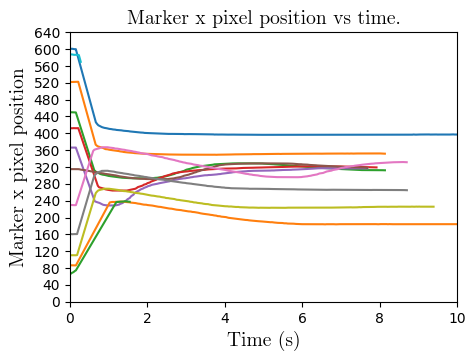
\includegraphics[width=\textwidth]{images/jetson_gimbal_performance_x_axis.png}
    \caption{Performance of the Jetson drone aiming the gimbal in the x axis.}
    \label{fig:jetson_gimbal_performance_x_axis}
    \end{subfigure}
    \begin{subfigure}[b]{0.49\textwidth}
        \centering
        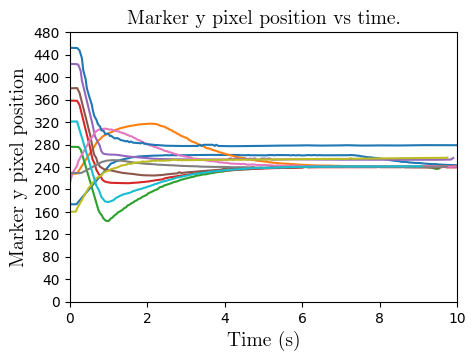
\includegraphics[width=\textwidth]{images/jetson_gimbal_performance_y_axis.png}
    \caption{Performance of the Jetson drone aiming the gimbal in the y axis.}
    \label{fig:jetson_gimbal_performance_y_axis}
    \end{subfigure}
        \begin{subfigure}[b]{0.49\textwidth}
        \centering
        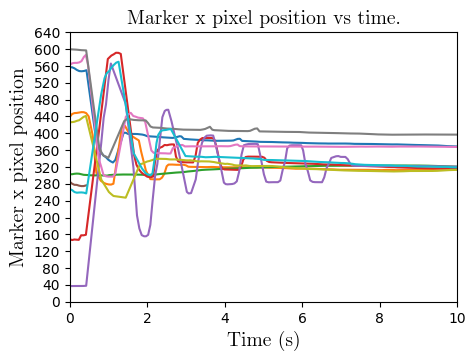
\includegraphics[width=\textwidth]{images/coral_gimbal_performance_x_axis.png}
    \caption{Performance of the Coral drone aiming the gimbal in the x axis.}
    \label{fig:coral_gimbal_performance_x_axis}
    \end{subfigure}
    \begin{subfigure}[b]{0.49\textwidth}
        \centering
        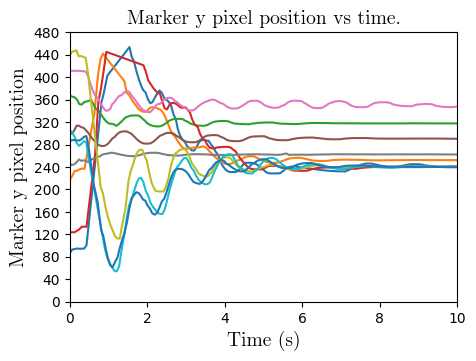
\includegraphics[width=\textwidth]{images/coral_gimbal_performance_y_axis.png}
    \caption{Performance of the Coral drone aiming the gimbal in the y axis.}
    \label{fig:coral_gimbal_performance_y_axis}
    \end{subfigure}
    \caption{Performance of aiming the gimbals.}
    \label{fig:gimbal_aim_performance}
\end{figure}

% \begin{figure}
%     \centering
%     \includegraphics[width=0.9\textwidth]{images/gimbal_performance_x_axis.png}
%     \caption{Performance of aiming the gimbal in the x axis.}
%     \label{fig:gimbal_performance_x_axis}
% \end{figure}

% \begin{figure}
%     \centering
%     \includegraphics[width=0.9\textwidth]{images/gimbal_performance_y_axis.png}
%     \caption{Performance of aiming the gimbal in the y axis.}
%     \label{fig:gimbal_performance_y_axis}
% \end{figure}